\subsection{Phase portrait analysis}

Being
\begin{equation*}
	q=
	\frac{a_{1}b_{3}}{b_{1}\left(c-a_{3}\right)}.
\end{equation*}
Considering
\begin{equation*}
	q>0\iff
	c-a_{3}>0\iff
	c>a_{3}.
\end{equation*}
Given the system~\eqref{eq:system}.
Setting $\diff{\theta}{\xi}=0$ and if $c-a_{1}S_{\text{o}}\neq 0$,
$c-a_{3}\neq 0$ and~\eqref{Sy}, then
\begin{equation*}
	S_{\text{o}}\left(S^{\text{R}}_{\text{o}}-S_{\text{o}}\right)=
	\left[
		\frac{\beta\theta\left(c-a_{3}\right)}{b_{1}\left(c-a_{3}\right)-a_{1}b_{3}\theta}
		\right]
	\frac{S^{\text{R}}_{\text{o}}}{S^{\text{L}}_{\text{y}}}
	\frac{1}{\Phi\left(\theta\right)}.
\end{equation*}

\subsubsection{The curve $\Gamma$}

Letting
\begin{equation*}
	f\left(\theta\right)\coloneqq
	\left[
		\frac{\beta\theta\left(c-a_{3}\right)}{b_{1}\left(c-a_{3}\right)-a_{1}b_{3}\theta}
		\right]
	\frac{S^{R}_{\text{o}}}{S^{L}_{y}}
	\frac{1}{\Phi\left(\theta\right)}.
	% \exp\left(\frac{E_{r}}{R\left(T^{\ast}\theta+T_{\text{res}}\right)}\right)
\end{equation*}
We define the curve $\Gamma$ as follows
\begin{equation*}
	\Gamma=
	\left\{
	\left(S_{\text{o}},\theta\right)\mid
	S_{\text{o}}
	\big(
	S^{\text{R}}_{\text{o}}-
	S_{\text{o}}
	\big)=
	f\left(\theta\right),\theta\geq0
	\right\}.
\end{equation*}
Letting
\begin{equation*}
	m\coloneqq
	\frac{\beta S^{\text{R}}_{\text{o}}}{b_{1}S^{\text{L}}_{\text{y}}t^{\ast}k_{p}},\quad
	\varepsilon\coloneqq
	\frac{E_{\text{r}}}{RT^{\ast}},\qquad
	\theta_{0}\coloneqq
	\frac{T_{\text{res}}}{T^{\ast}},\qquad
	q\coloneqq
	\frac{a_{1}b_{3}}{b_{1}\left(c-a_{3}\right)}.
\end{equation*}
We obtain
\begin{equation*}
	f\left(\theta\right)=
	\frac{m\theta}{1-q\theta}
	\exp\left(\frac{\varepsilon}{\theta+\theta_{0}}\right),\quad\theta\neq\frac{1}{q}.
\end{equation*}
From the function given above, we have two cases to analyze.
\begin{itemize}
	\item If $\theta<\frac{1}{q}$, then $f\left(\theta\right)>0$.
	\item If $\theta>\frac{1}{q}$, then $f\left(\theta\right)<0$.
\end{itemize}
Therefore, by analyzing the asymptotes of $f\left(\theta\right)$, we have that $-\frac{m}{q}$ is a horizontal asymptote
and $\frac{1}{q}$ is a vertical asymptote.
On the other hand, taking into account
\begin{equation*}
	\diff{f\left(\theta\right)}{\theta}=
	m
	\left[
		\frac{
			\left(1+q\varepsilon\right)\theta^{2}+\left(2\theta_{0}-\varepsilon\right)\theta+\theta_{0}^{2}}{
			\left(1-q\theta\right)^{2}\left(\theta+\theta_{0}\right)^{2}
		}
		\right]
	\exp\left(\frac{\varepsilon}{\theta+\theta_{0}}\right).
\end{equation*}
Since we want to analyze the behavior of $f\left(\theta\right)$, we analyze the polynomial
\begin{equation*}
	p\left(\theta\right)\coloneqq
	\left(1+q\varepsilon\right)\theta^{2}+\left(2\theta_{0}-\varepsilon\right)\theta+\theta_{0}^{2}.
\end{equation*}
Since $1+q\varepsilon>1>0$, and if we consider the x-coordinate of the parabola's vertex as follows
$h=-\frac{2\theta_{0}-\varepsilon}{2\left(1+q\varepsilon\right)}=\frac{\varepsilon-2\theta_{0}}{2\left(1+q\varepsilon\right)}$
and taking into account the discriminant
\begin{math}
	\Delta=
	{\left(2\theta_{0}-\varepsilon\right)}^{2}-
	4\left(1+q\varepsilon\right)
	\theta_{0}^{2}=
	\varepsilon
	\left[
		\varepsilon-
		\left(4\theta_{0}+4q\theta^{2}_{0}\right)
		\right]
\end{math}
of $p\left(\theta\right)=0$.
In the graphs of $\theta$ versus $f\left(\theta\right)$, the ordered pair $\left(\theta_{\text{M}},S^{\ast}_{\text{o}}\right)$ is considered,
where $S^{\ast}_{\text{o}}=f\left(\theta_{\text{M}}\right)=\frac{{\left(S^{\text{R}}_{\text{o}}\right)}^{2}}{4}$.
To create the graphs, we have the following results for both $f\left(\theta\right)$ and its respective phase diagram.
\begin{figure}[ht!]
	\centering
	\begin{subfigure}[ht!]{0.35\textwidth}
		\centering
		\includegraphics[width=\linewidth]{q_p_delt_neg_h_neg}
		\caption{$q>0$, $\Delta<0$, $\varepsilon<2\theta_{0}$.}
	\end{subfigure}
	\hfill
	\begin{subfigure}[ht!]{0.35\textwidth}
		\centering
		\includegraphics[width=\linewidth]{q_p_delt_neg_h_neg}
		\caption{$q>0$, $\Delta<0$, $\varepsilon=2\theta_{0}$.}
	\end{subfigure}
	\vspace{0.5em}
	\begin{subfigure}[ht!]{0.35\textwidth}
		\centering
		\includegraphics[width=\linewidth]{q_p_delt_neg_h_neg}
		\caption{$q>0$, $\Delta<0$, $\varepsilon>2\theta_{0}$.}
	\end{subfigure}
	\hfill
	\begin{subfigure}[ht!]{0.35\textwidth}
		\centering
		\includegraphics[width=\linewidth]{q_p_delt_zero_h_posit}
		\caption{$q>0$, $\Delta=0$, $\varepsilon>2\theta_{0}$.}
	\end{subfigure}
	\vspace{0.8em}
	% fila 3 (imagen centrada ocupando ancho)
	\begin{subfigure}[ht!]{0.35\textwidth}
		\centering
		\includegraphics[width=\linewidth]{q_p_delt_posit_h_posit_1}
		\caption{$q>0$, $\Delta>0$, $\varepsilon>2\theta_{0}$, $S^{\ast}_{\text{o}}<f\left(\theta_{2}\right)<f\left(\theta_{1}\right)$.}
	\end{subfigure}
	\caption{$f\left(\theta\right)$ with the same $\theta$ vs $S_{\text{o}}$ representation.}
	\label{fig:5en221}
\end{figure}

\begin{figure}[ht!]
	\centering
	\begin{tikzpicture}[scale=0.75]
		% Ejes
		\draw[->] (-3,0) -- (6.5,0) node[anchor=north] {$S_o$};
		\draw[->] (0,-2) -- (0,6) node[anchor=east] {$\theta$};
		% Parábola hacia abajo: y = a*x*(S_o^R - x)
		\draw[thick, blue, domain=-0.9:4.9, samples=100]
		plot(\x,{0.5*\x*(4 - \x)}) node at (3,1.8) {$\Gamma$};
		%hiperbolas
		\draw[domain=-2.75:-1.25,smooth,variable=\x,blue,thick]
		plot ({\x},{ -0.5/( \x +1)+3 });
		\draw[domain=5.25:6.5,smooth,variable=\x,blue,thick]
		plot ({\x},{ 0.5/( \x -5)+3 });
		%plot ({\x},{(1.75)*(\x+2.75)^2 + 3});
		%   \node at (3,1.8) {$\Gamma$};
		% Etiquetas de los puntos
		\node[below left] at (0,0) {$0$};
		\node[below] at (4,0) {$S^{\text{R}}_{\text{o}}$};
		%\node[below] at (2,0) {$\dfrac{S_o^R}{2}$};
		\node[below] at (-0.25,2) {$\theta_{\text{M}}$};
		%\node[below left] at (0,0) {$(0,0)$};
		%\node[below] at (4,0) {$(S_o^R,0)$};
		% Línea vertical punteada en x = -1 y 5
		\draw[dashed] (5,-3.) -- (5,5);
		\draw[dashed] (-1,-3) -- (-1,5);
		% Línea horizontal punteada en y=3
		\draw[blue, dashed] (-3,3) -- (6.25,3);
		\node[below] at (-.25,3.5) {$\frac{1}{q}$};
		\draw[red, thick] (4,-2.5) -- (4,4);
		\draw[red, thick] (0,-2.5) -- (0,4);
		%\draw[dashed] (2,0) -- (2,2);
		%\draw[dashed] (0,2) -- (2,2);
	\end{tikzpicture}
\end{figure}
When $f\left(\theta\right)$ is
\begin{figure}[ht!]
	\centering
	\includegraphics[width=0.4\textwidth]{q_p_delt_posit_h_posit_2}
	\caption{$q>0$, $\Delta>0$, $\varepsilon>2\theta_{0}$, $f\left(\theta_{2}\right)<S^{\ast}_{\text{o}}<f\left(\theta_{1}\right)$.}
	%	\label{q_p_delt_posit_h_posit_2}
\end{figure}
The representation $\theta$ vs $S_{\text{o}}$  is
\begin{figure}[ht!]
	\centering
	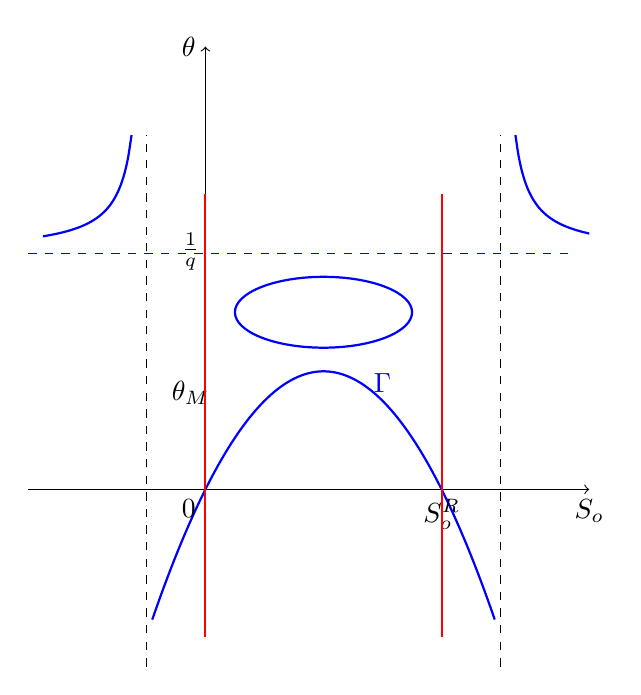
\begin{tikzpicture}[scale=0.75]
		\draw[->] (-3,0) -- (6.5,0) node[anchor=north] {$S_{\text{o}}$};
		\draw[->] (0,-2) -- (0,7.5) node[anchor=east] {$\theta$};
		% Parábola hacia abajo: y = a*x*(S_o^R - x)
		\draw[thick, blue, domain=-0.9:4.9, samples=100]
		plot(\x,{0.5*\x*(4 - \x)}) node at (3,1.8) {$\Gamma$};
		%elipse
		\draw[thick,blue] (2,3) ellipse [x radius=1.5, y radius=0.6];
		%hiperbolas
		\draw[domain=-2.75:-1.25,smooth,variable=\x,blue,thick]
		plot ({\x},{ -0.5/( \x +1)+4 });
		\draw[domain=5.25:6.5,smooth,variable=\x,blue,thick]
		plot ({\x},{ 0.5/( \x -5)+4 });
		%plot ({\x},{(1.75)*(\x+2.75)^2 + 3});
		%   \node at (3,1.8) {$\Gamma$};
		% Etiquetas de los puntos
		\node[below left] at (0,0) {$0$};
		\node[below] at (4,0) {$S^{\text{R}}_{\text{o}}$};
		%\node[below] at (2,0) {$\dfrac{S_o^R}{2}$};
		\node[below] at (-0.25,2) {$\theta_{M}$};
		%\node[below left] at (0,0) {$(0,0)$};
		%\node[below] at (4,0) {$(S_o^R,0)$};
		% Línea vertical punteada en x = -1 y 5
		\draw[dashed] (5,-3.) -- (5,6);
		\draw[dashed] (-1,-3) -- (-1,6);
		% Línea horizontal punteada en y=4
		\draw[blue, dashed] (-3,4) -- (6.25,4);
		\node[below] at (-.25,4.5) {$\frac{1}{q}$};
		\draw[red, thick] (4,-2.5) -- (4,5);
		\draw[red, thick] (0,-2.5) -- (0,5);
		%\draw[dashed] (2,0) -- (2,2);
		%\draw[dashed] (0,2) -- (2,2);
	\end{tikzpicture}
\end{figure}
and the $f\left(\theta\right)$ graph
\begin{figure}[ht!]
	\centering
	\includegraphics[width=0.45\textwidth]{q_p_delt_posit_h_posit_3}
	\caption{$q>0$, $\Delta>0$, $\varepsilon>2\theta_{0}$, $f\left(\theta_{2}\right)<f\left(\theta_{1}\right)<S^{\ast}_{\text{o}}$.}
	\label{q_pos_delt_posit_varep_2theta_f}
\end{figure}
has the $\theta$ vs $S_{\text{o}}$ representation
\begin{figure}[ht!]
	\centering
	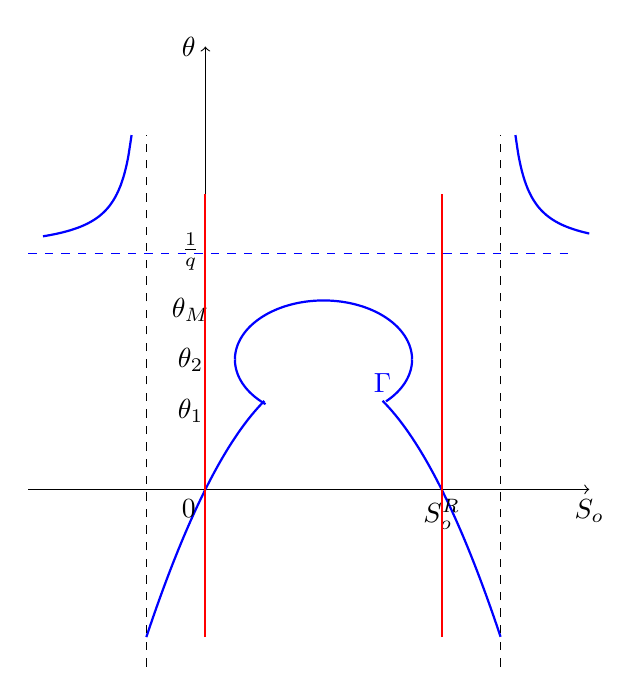
\begin{tikzpicture}[scale=0.75]
		% Ejes
		\draw[->] (-3,0) -- (6.5,0) node[anchor=north] {$S_{\text{o}}$};
		\draw[->] (0,-2) -- (0,7.5) node[anchor=east] {$\theta$};
		% Parábola hacia abajo: y = a*x*(S_o^R - x)
		\draw[thick, blue, domain=-1:1, samples=100]
		plot(\x,{0.5*\x*(4 - \x)}) ;
		\draw[thick, blue, domain=3:5, samples=100]
		plot(\x,{0.5*\x*(4 - \x)}) node at (3,1.8) {$\Gamma$};
		% Parte izquierda inferior
		\draw[thick, blue, samples=50, domain=180:130.87]
		plot ({2. + 1.5*cos(\x)}, {2.2 - 1*sin(\x)});
		% Parte superior completa
		\draw[thick, blue, samples=100, domain=0:180]
		plot ({2. + 1.5*cos(\x)}, {2.2 + 1*sin(\x)});
		% Parte derecha inferior
		\draw[thick, blue, samples=50, domain=45.13:0]
		plot ({2. + 1.5*cos(\x)}, {2.2 - 1*sin(\x)});
		%hiperbolas
		\draw[domain=-2.75:-1.25,smooth,variable=\x,blue,thick]
		plot ({\x},{ -0.5/( \x +1)+4 });
		\draw[domain=5.25:6.5,smooth,variable=\x,blue,thick]
		plot ({\x},{ 0.5/( \x -5)+4 });
		%plot ({\x},{(1.75)*(\x+2.75)^2 + 3});
		%   \node at (3,1.8) {$\Gamma$};
		% Etiquetas de los puntos
		\node[below left] at (0,0) {$0$};
		\node[below] at (4,0) {$S_o^R$};
		%\node[below] at (2,0) {$\dfrac{S_o^R}{2}$};
		\node[below] at (-0.25,1.7) {$\theta_{1}$};
		\node[below] at (-0.25,2.55) {$\theta_{2}$};
		\node[below] at (-0.25,3.4) {$\theta_{\text{M}}$};
		%\node[below left] at (0,0) {$(0,0)$};
		%\node[below] at (4,0) {$(S_o^R,0)$};
		% Línea vertical punteada en x = -1 y 5
		\draw[dashed] (5,-3.) -- (5,6);
		\draw[dashed] (-1,-3) -- (-1,6);
		% Línea horizontal punteada en y=4
		\draw[blue, dashed] (-3,4) -- (6.25,4);
		\node[below] at (-.25,4.5) {$\frac{1}{q}$};
		\draw[red, thick] (4,-2.5) -- (4,5);
		\draw[red, thick] (0,-2.5) -- (0,5);
		%\draw[dashed] (2,0) -- (2,2);
		%\draw[dashed] (0,2) -- (2,2);
	\end{tikzpicture}
\end{figure}
We determined the phase diagram of the system
\begin{equation*}
	\left\{
	\begin{aligned}
		\diff{S_{\text{o}}}{\xi} & =
		F_{1}\left(S_{\text{o}},\theta\right). \\
		\diff{\theta}{\xi}       & =
		F_{2}\left(S_{\text{o}},\theta\right).
	\end{aligned}
	\right.
\end{equation*}
for all the $f\left(\theta\right)$ graphs.
Where
\begin{align*}
	F_{1}
	\left(S_{\text{o}},\theta\right) & =
	\frac{b_{3}S^{\text{L}}_{\text{y}}
		\Phi\left(\theta\right)
		\left(S^{\text{R}}_{\text{o}}-S_{\text{o}}\right)S_{\text{o}}}{S^{\text{R}}_{\text{o}}\left(c-a_{3}\right)},
	\shortintertext{and}
	F_{2}
	\left(S_{\text{o}},\theta\right) & =
	\frac{
		b_{1}
		\left(1-q\theta\right)
		\Phi\left(\theta\right)
		S^{\text{L}}_{\text{y}}
		\left[
			S^{2}_{\text{o}}-
			S^{\text{R}}_{\text{o}}S_{\text{o}}+
			f\left(\theta\right)
			\right]
	}{
		\left(c-a_{1}S_{\text{o}}\right)
		S^{\text{R}}_{\text{o}}
	}.
\end{align*}

\newpage
To verify the specific case we are analyzing, we perform the following calculations.
In our case
\begin{itemize}
	\item $q=6.54979\times 10^{-5}$.
	\item $\Delta=298.866$
	\item  $\varepsilon = 20.5465$
	\item 	$\theta_0 =1.5 $
	\item $S_o^R=1$
	\item $  S_o^* = \dfrac{  ( S_o^R)^2 }{4}  = \dfrac{1}{4}=0.25$
	\item $ f(\theta_1)= 0.000000157446 $
	\item $ f(\theta_2)= 0.000000000210 $
\end{itemize}
So

$q>0$, $\Delta>0$, $\varepsilon>2\theta_{0}$,
$f(\theta_2)<f(\theta_{1})<S_{\text{o}}^{\ast}$

this corresponds to the case \ref{num_case}

Besides
\[  \dfrac{c}{a_1} = 15235.9  \]

Then the flux diagram

\begin{center}
	\begin{tikzpicture}[scale=1.2]
		% Ejes
		\draw[->] (-3,0) -- (9,0) node[anchor=north] {$S_o$};
		\draw[->] (0,-2) -- (0,7.5) node[anchor=east] {$\theta$};
		% Parábola hacia abajo: y = a*x*(S_o^R - x)
		\draw[thick, blue, domain=-1:1, samples=100]
		plot(\x,{0.5*\x*(4 - \x)}) ;
		\draw[thick, blue, domain=3:5, samples=100]
		plot(\x,{0.5*\x*(4 - \x)}) node at (3,1.8) {$\Gamma$};
		% Parte izquierda inferior
		\draw[thick, blue, samples=50, domain=180:130.87]
		plot ({2. + 1.5*cos(\x)}, {2.2 - 1*sin(\x)});
		% Parte superior completa
		\draw[thick, blue, samples=100, domain=0:180]
		plot ({2. + 1.5*cos(\x)}, {2.2 + 1*sin(\x)});
		% Parte derecha inferior
		\draw[thick, blue, samples=50, domain=45.13:0]
		plot ({2. + 1.5*cos(\x)}, {2.2 - 1*sin(\x)});
		%hiperbolas
		\draw[domain=-2.75:-1.25,smooth,variable=\x,blue,thick]
		plot ({\x},{ -0.5/( \x +1)+4 });
		\draw[domain=5.9:8.5,smooth,variable=\x,blue,thick]
		plot ({\x},{ 0.5/( \x -5.7)+4 });
		%plot ({\x},{(1.75)*(\x+2.75)^2 + 3});
		%   \node at (3,1.8) {$\Gamma$};
		% Etiquetas de los puntos
		\node[below left] at (0,0) {$0$};
		\node[below] at (4,0) {$S_o^R$};
		%\node[below] at (2,0) {$\dfrac{S_o^R}{2}$};
		\node[below] at (-0.25,1.7) {$\theta_1 $};
		\node[below] at (-0.25,2.55) {$\theta_2 $};
		\node[below] at (-0.25,3.4) {$\theta_M $};
		%\node[below left] at (0,0) {$(0,0)$};
		%\node[below] at (4,0) {$(S_o^R,0)$};
		% Línea vertical punteada en x = -1 y 5.75
		\draw[dashed] (5.75,-3.) -- (5.75,6.5);
		\draw[dashed] (-1,-3) -- (-1,6.5);
		% Línea vertical punteada en S_o=c/a_1
		\draw[red, dashed] (6.85,-1.75) -- (6.85,6.25);
		\node[below] at (6.85,-1.75) {$S_o=\dfrac{c}{a_1}$};
		% Línea horizontal punteada en y=4
		\draw[blue, dashed] (-3,4) -- (8.5,4);
		\node[below] at (-.25,4.5) {$1/q$};
		\draw[red, thick] (4,-2.5) -- (4,5);
		\draw[red, thick] (0,-2.5) -- (0,5);
		%\draw[dashed] (2,0) -- (2,2);
		%\draw[dashed] (0,2) -- (2,2);
		% Diagram arrows
		%A_1
		\draw[->,line width=2pt, shorten >=2pt](-0.3,0.25) -- (-0.9,0.25);
		\draw[->,line width=2pt, shorten >=2pt] (-.3,0.25) -- (-0.3,0.85);
		\draw[->,line width=2pt, shorten >=2pt] (-0.45,-0.75) -- (-0.45,-0.2);
		\draw[->,line width=2pt, shorten >=2pt](-0.45,-0.75) -- (-0.95,-0.75);
		%A_2
		\draw[->,line width=2pt, shorten >=2pt](0.2,1.25) -- (0.7,1.25);
		\draw[->,line width=2pt, shorten >=2pt] (0.2,1.25) -- (0.2,1.75);
		%	\draw[->,line width=2pt, shorten >=2pt](2.5,2.25) -- (3,2.25);
		%	\draw[->,line width=2pt, shorten >=2pt] (2.5,2.25) -- (2.5,2.75);
		\draw[->,line width=2pt, shorten >=2pt](2.0,3.45) -- (2.5,3.45);
		\draw[->,line width=2pt, shorten >=2pt] (2.0,3.45) -- (2.0,3.85);
		\draw[->,line width=2pt, shorten >=2pt](3.45,1.35) -- (3.95,1.35);
		\draw[->,line width=2pt, shorten >=2pt] (3.45,1.35) -- (3.45,1.85);
		%A_3
		\draw[->,line width=2pt, shorten >=2pt](4.55,0.7) -- (4.05,0.7);
		\draw[->,line width=2pt, shorten >=2pt] (4.55,0.7) -- (4.55,1.5);
		\draw[->,line width=2pt, shorten >=2pt](8.3 ,1.3) -- (7.8 ,1.3);
		\draw[->,line width=2pt, shorten >=2pt] (8.3 ,1.3) -- (8.3 ,0.6);
		\draw[->,line width=2pt, shorten >=2pt](8.3 ,-0.7) -- (7.8 ,-0.7);
		\draw[->,line width=2pt, shorten >=2pt] (8.3 ,-0.7) -- (8.3 ,-1.5);
		\draw[->,line width=2pt, shorten >=2pt](6.55,0.7) -- (6.05,0.7);
		\draw[->,line width=2pt, shorten >=2pt] (6.55,0.7) -- (6.55,1.5);
		\draw[->,line width=2pt, shorten >=2pt](6.55,-1.5) -- (6.05,-1.5);
		\draw[->,line width=2pt, shorten >=2pt] (6.55,-1.5) -- (6.55,-0.7);
		%U_1
		\draw[->,line width=2pt, shorten >=2pt] (-0.15,-1.75) -- (-0.15,-2.35);
		\draw[->,line width=2pt, shorten >=2pt](-0.15,-1.75) -- (-0.65,-1.75);
		%U_2^l
		\draw[->,line width=2pt, shorten >=2pt] (0.95,0.75) -- (0.95,0.2);
		\draw[->,line width=2pt, shorten >=2pt](0.95,0.75) -- (1.45,0.75);
		\draw[->,line width=2pt, shorten >=2pt] (0.95,-0.5) -- (0.95,-1.25);
		\draw[->,line width=2pt, shorten >=2pt](0.95,-0.5) -- (1.45,-0.5);
		%U_2^r
		\draw[->,line width=2pt, shorten >=2pt](2.5,1.25) -- (3,1.25);
		\draw[->,line width=2pt, shorten >=2pt] (2.5,1.25)
		-- (2.5,0.5);
		\draw[->,line width=2pt, shorten >=2pt](3.25,-0.35) -- (3.75,-0.35);
		\draw[->,line width=2pt, shorten >=2pt] (3.25,-0.35)
		-- (3.25,-1.05);
		% U_3
		\draw[->,line width=2pt, shorten >=2pt] (4.4,-1.15) -- (4.4,-1.65);
		\draw[->,line width=2pt, shorten >=2pt](4.4,-1.15) -- (4.01,-1.15);
		%over 1/q similar to U
		\draw[->,line width=2pt, shorten >=2pt] (-0.15,4.95) -- (-0.15,4.45);
		\draw[->,line width=2pt, shorten >=2pt](-0.15,4.95) -- (-0.65,4.95);
		\draw[->,line width=2pt, shorten >=2pt] (0.95,4.95) -- (0.95,4.45);
		\draw[->,line width=2pt, shorten >=2pt](0.95,4.95) -- (1.45,4.95);
		\draw[->,line width=2pt, shorten >=2pt](2.5,4.95) -- (3,4.95);
		\draw[->,line width=2pt, shorten >=2pt] (2.5,4.95) -- (2.5,4.45);
		\draw[->,line width=2pt, shorten >=2pt] (4.8,4.95) -- (4.8,4.45);
		\draw[->,line width=2pt, shorten >=2pt](4.8,4.95) -- (4.41,4.95);
		\draw[->,line width=2pt, shorten >=2pt] (6.3,4.55) -- (6.3,4.05);
		\draw[->,line width=2pt, shorten >=2pt](6.3,4.55) -- (5.81,4.55);
		\draw[->,line width=2pt, shorten >=2pt] (6.5,5.45) -- (6.5,5.95);
		\draw[->,line width=2pt, shorten >=2pt](6.5,5.45) -- (6.1,5.45);
		\draw[->,line width=2pt, shorten >=2pt] (7.9,5.95) -- (7.9,5.45);
		\draw[->,line width=2pt, shorten >=2pt](7.9,5.95) -- (7.51,5.95);
		%ellipse  similar to under
		\draw[->,line width=2pt, shorten >=2pt](1.75,2.75) -- (2.25,2.75);
		\draw[->,line width=2pt, shorten >=2pt] (1.75,2.75) -- (1.75,2.25);
	\end{tikzpicture}
\end{center}

According to the phase diagram we have
\begin{itemize}
	\item OC:$\left(0,0\right)$ is a repulsor point.
	\item FC:$\left(S^{\text{R}}_{\text{o}},0\right)$ is a saddle point.
\end{itemize}

We found two cases
\begin{itemize}
	\item  If  $\dfrac{c}{a_1} < S_o^R$
	      \begin{itemize}
		      \item $OC : (0,0)  $ is a repulsor.
		      \item   $FC : (S_o^R,0)  $ is an  atractor.
	      \end{itemize}
	      which coincides with the eigenvalue analysis.


	\item If  $   S_o^R   < \dfrac{c}{a_1}$
	      \begin{itemize}
		      \item $OC : (0,0)  $ is a repulsor.
		      \item   $FC : (S_o^R,0)  $ is a   saddle.
	      \end{itemize}
	      which coincides with the eigenvalue analysis.
\end{itemize}

% On the other hand, for physical criteria $q>0$.
% Next, we plot $\theta\mapsto f\left(\theta\right)$ and the phase portrait.
% TODO: Comment on Figure 1, Figure 5, Figure 7, and Figure 9.
% Comment: Numerical Analysis
% TODO: Before the Gamma curve, place the ODE.

% TODO: Add an introduction to the Gamma curve, rewriting the original ODEs for Sy' and theta'. By rewriting using f(theta), it is observed that to determine the phase diagram, it is necessary to know the behavior of f(theta).
% Considering q>0, the following phase diagram is obtained, and a source and a saddle are observed.
% \begin{equation*}
% 	F\left(S_{\text{o}},\theta\right)=
% 	\begin{bmatrix}
% 		F_{1}\left(S_{\text{o}},\theta\right) \\
% 		F_{2}\left(S_{\text{o}},\theta\right)
% 	\end{bmatrix}=
% 	\begin{bmatrix}\displaystyle
% 		\frac{b_{3}S_{\text{y}}S_{\text{o}}}{c-a_{3}}
% 		\Phi\left(\theta\right) \\
% 		\displaystyle
% 		\frac{
% 			\beta\theta
% 			\left(c-a_{3}\right)+
% 			\left[
% 				a_{1}
% 				b_{3}
% 				\theta-
% 				b_{1}
% 				\left(c-a_{3}\right)
% 				\right]
% 			S_{\text{o}}
% 			S_{\text{y}}
% 			\Phi\left(\theta\right)}{
% 			\left(c-a_{1}S_{\text{o}}\right)
% 			\left(c-a_{3}\right)
% 		}
% 	\end{bmatrix}.
% \end{equation*}
%Beside
%\[    f(\theta)  =  \dfrac{ m \theta }{1-q \theta } e^{ \varepsilon/ \theta + \theta_0 }  > 0     \]
% For $f(\theta)$ analysis we need $f'(\theta)$ and his discriminant $\Delta$.
%So the next cases, the most important fact is than
%\[   S_o^* < -\dfrac{m}{q} \]

% Let us analyze when system \eqref{ec35c}-\eqref{ec39c} possesses a solution satisfying limits \eqref{eq:limits} and \eqref{eq:Riemann_boundary}.
% \begin{theorem}
% 	\label{teo4}
% 	Assuming $c > a_1$ and $c > a_3$ then there exists a solution of system \eqref{ec35c}-\eqref{ec39c} satisfying the limits \eqref{eq:limits}, \eqref{eq:Riemann_boundary}.
% \end{theorem}

% \begin{theorem}
% 	\label{t:domain}
% 	Consider $c > a_1$, $c < a_2$, and $c > a_3$. The solution of system \eqref{ec35c}-\eqref{ec39c} satisfying the limits \eqref{eq:limits}, \eqref{eq:Riemann_boundary} with initial condition in the physical domain $S_o\in [0,1]$, $S_y\in [0,1]$, $\theta\in [0,\infty)$ stays inside this physical domain.
% \end{theorem}

\subsection{Existence and uniqueness of solution}

Taking into account the results of Section 3.2, where $JF_{\text{OC}}$,
$JF_{\text{FC}}$ and their respective eigenvalues $\lambda^{OC}_{1}$, $\lambda^{OC}_{2}$, $\lambda^{FC}_{1}$, $\lambda^{FC}_{2}$ were determined.
The linearization of system \eqref{eq:system} at the point $\left(S_{\text{o}},\theta\right)$ yields the derivative matrix  $JF\left(S_{\text{o}},\theta\right)$.

For the non-resonant case both equilibrium are strictly hyperbolic
allowing to prove the following proposition.

\begin{proposition}
	In the case $c\neq a_{3}$ and $c\neq a_{1}S_{\text{o}}^{\text{R}}$,
	there exists a unique traveling combustion wave solution for system
	\eqref{eq:14}-\eqref{eq:16}.
\end{proposition}

\begin{proposition}
	For the resonance case $c=a_{3}\vee c=a_{1}S_{\text{o}}^{\text{R}}$,
	system \eqref{eq:14}-\eqref{eq:16} possesses a unique traveling combustion wave
	solution if and only if there is $\theta_{M}>0$ such that
	$4f\left(\theta_{M}\right)=\left(S_{\text{o}}^{\text{R}}\right)^2$
	with $f$ strictly increasing on $0\leq\theta\leq\theta_{M}$.
\end{proposition}

\subsection{Without heat losses}

By setting $\beta=0$ in systems (15) to (18) and considering
conditions (13) and (14), we obtain the following results:
\begin{equation}
	\label{eq:theta_nl}
	-c\diff{\theta}{\xi}+
	a_{1}\diff{\left(S_{\text{o}}\theta\right)}{\xi}=
	b_{1}S_{\text{o}}S_{\text{y}}\Phi\left(\theta\right),
\end{equation}
\begin{equation}
	\label{eq:Sy_nl}
	\left(a_{2}-c\right)\diff{S_{\text{y}}}{\xi}=
	-b_{2}S_{\text{o}}S_{\text{y}}\Phi\left(\theta\right),
\end{equation}
\begin{equation}
	\label{eq:So_nl}
	\left(a_{3}-c\right)\diff{S_{\text{o}}}{\xi}=
	-b_{3}S_{\text{o}}S_{\text{y}}\Phi\left(\theta\right).
\end{equation}

We find:
\begin{equation*}
	\theta^{\text{L}}=
	\theta^{\text{R}}
	\left(
	\frac{c-a_{1}S_{\text{o}}^{\text{R}}}{c}
	\right)-
	\frac{\left(a_{3}-a_{2}\right)b_{1}S_{\text{o}}^{\text{R}}S_{\text{y}}^{\text{L}}}{a_{2}b_{3}S_{\text{y}}^{\text{L}}+a_{3}b_{2}S_{\text{o}}^{\text{R}}},
\end{equation*}

\begin{equation*}
	\theta=
	\theta^{\text{R}}
	\left(\frac{c-a_{1}S_{\text{o}}^{\text{R}}}{c-a_{1}S_{\text{o}}}\right)-
	\frac{b_{1}}{b_{2}}
	\left(\frac{c-a_{2}}{c-a_{1}S_{\text{o}}}\right)
	\left(S_{\text{o}}^{\text{R}}-S_{\text{o}}\right)
	\frac{S_{\text{y}}^{\text{L}}}{S_{\text{o}}^{\text{R}}}.
\end{equation*}

To find the traveling wave solution of the system~\eqref{eq:theta_nl}-\eqref{eq:So_nl}
is equivalent to finding the solution of the system composed of one ODE
\begin{equation}
	\label{eq:So_ode_nl}
	\diff{S_{\text{o}}}{\xi}=
	\frac{b_{3}S_{\text{o}}S_{\text{y}}}{c-a_{3}}
	\Phi\left(\theta\right),
\end{equation}
and two algebraic equations
\begin{equation}
	\label{eq:Sy_alg_nl}
	S_{\text{y}}=
	\left(S_{\text{o}}^{\text{R}}-S_{\text{o}}\right)
	\frac{S_{\text{y}}^{\text{L}}}{S_{\text{o}}^{\text{R}}}
\end{equation}
and
\begin{equation}
	\label{eq:theta_alg_nl}
	\theta=
	\theta^{\text{R}}
	\left(\frac{c-a_{1}S_{\text{o}}^{\text{R}}}{c-a_{1}S_{\text{o}}}\right)-
	\frac{b_{1}}{b_{2}}
	\left(\frac{c-a_{2}}{c-a_{1}S_{\text{o}}}\right)
	\left(S_{\text{o}}^{\text{R}}-S_{\text{o}}\right)
	\frac{S_{\text{y}}^{\text{L}}}{S_{\text{o}}^{\text{R}}}.
\end{equation}

% In this case, the Jacobian matrices at the equilibrium points OC and FC, denoted as $JF_{\text{OC}}$ and $JF_{\text{FC}}$, are given by:
% \begin{equation*}
% 	JF_{\text{OC}}=
% 	\begin{bmatrix}
% 		\frac{b_{3}e}{c-a_{3}} & 0 \\
% 		-\frac{b_{1}e}{c}      & 0
% 	\end{bmatrix},
% \end{equation*}
% \begin{equation*}
% 	JF_{\text{FC}}=
% 	\begin{bmatrix}
% 		-\frac{b_{3}e}{c-a_{3}}                & 0 \\
% 		\frac{b_{1}e}{c-a_{1}S^{R}_{\text{o}}} & 0
% 	\end{bmatrix}.
% \end{equation*}
% The corresponding eigenvalues are $\lambda^{1}_{\text{OC}}= \frac{b_{3}e}{c-a_{3}}$, $\lambda^{2}_{\text{OC}}= 0$ and $\lambda^{1}_{\text{FC}}= -\frac{b_{3}e}{c-a_{3}}$, $\lambda^{2}_{\text{FC}}= 0$.
% The fact that one of the eigenvalues is zero implies that the equilibrium points are non-hyperbolic, which distinguishes this case from the one with heat losses ($\beta > 0$).

Let us analyze when system \eqref{eq:theta_nl}-\eqref{eq:So_nl} possesses a solution satisfying limits \eqref{eq:limits} and \eqref{eq:Riemann_boundary}.
\begin{theorem}
	\label{teo4_nl}
	Assuming $c > a_1$ and $c > a_3$, then there exists a solution of system \eqref{eq:theta_nl}-\eqref{eq:So_nl} satisfying the limits \eqref{eq:limits}, \eqref{eq:Riemann_boundary}.
\end{theorem}

\begin{theorem}
	\label{t:domain_nl}
	Consider $c > a_1$, $c < a_2$, and $c > a_3$. The solution of system \eqref{eq:theta_nl}-\eqref{eq:So_nl} satisfying the limits \eqref{eq:limits}, \eqref{eq:Riemann_boundary} with initial condition in the physical domain $S_o\in [0,1]$, $S_y\in [0,1]$, $\theta\in [0,\infty)$ stays inside this physical domain.
\end{theorem}
